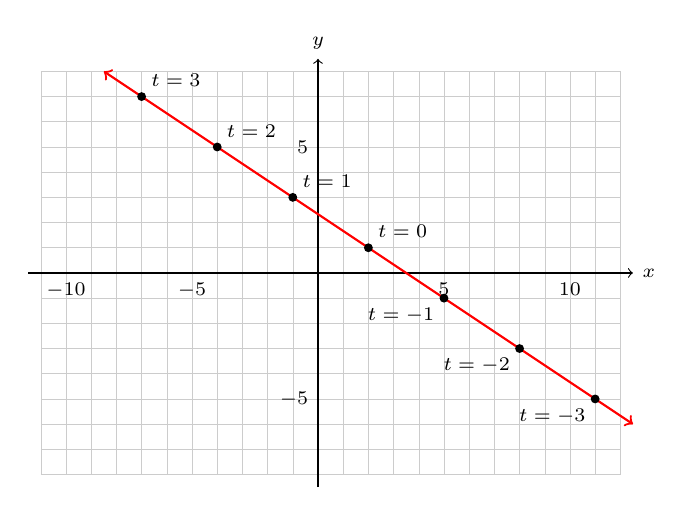
\begin{tikzpicture}[scale=0.32, every node/.style={font=\scriptsize}]
  \draw[gray!40, very thin] (-11,-8) grid (12,8);
  \draw[->] (-11.5,0) -- (12.5,0) node[right] {$x$};
  \draw[->] (0,-8.5) -- (0,8.5) node[above] {$y$};
  \foreach \x in {-10,-5,5,10} \node[below] at (\x,0) {$\x$};
  \foreach \y in {-5,5} \node[left] at (0,\y) {$\y$};
  \draw[red, thick, <->] (-8.5,8) -- (12.5,-6);
  \foreach \t in {-3,...,3} {
    \fill ({2-3*\t},{1+2*\t}) circle (5pt);
  }
  \node[above right] at (2,1) {$t=0$};
  \node[above right] at (-1,3) {$t=1$};
  \node[above right] at (-4,5) {$t=2$};
  \node[above right] at (-7,7) {$t=3$};
  \node[below left] at (5,-1) {$t=-1$};
  \node[below left] at (8,-3) {$t=-2$};
  \node[below left] at (11,-5) {$t=-3$};
\end{tikzpicture}
